\begin{figure}[t]
  \centering 
  \begin{minipage}{0.49\textwidth}
    \centering 

    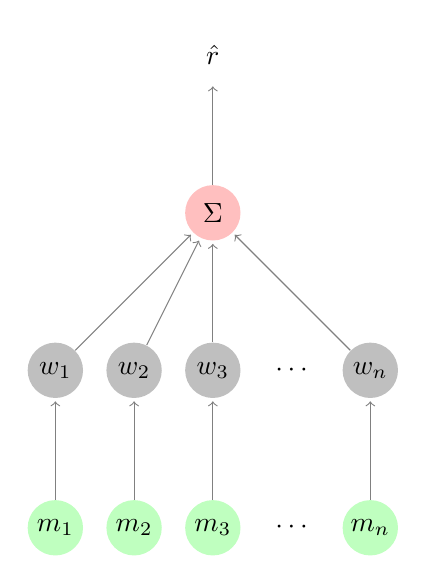
\begin{tikzpicture}[shorten >=1pt,->,draw=black!50, node distance=\layersep]
      \tikzstyle{every pin edge}=[<-,shorten <=2pt]
      \tikzstyle{node}=[circle,fill=black!25,minimum size=20pt,inner sep=0pt];
      \tikzstyle{method}=[node,fill=green!25];
      \tikzstyle{weight}=[node,fill=black!25];
      \tikzstyle{error}=[node,fill=blue!25];
      \tikzstyle{agg}=[node,fill=red!25];
      \tikzstyle{txt}=[node,fill=white];
       
      \node[method] (M1) at (0,-6) {$m_1$};      
      \node[method] (M2) at (1,-6) {$m_2$};         
      \node[method] (M3) at (2,-6) {$m_3$};         
      \node[txt]    (MS) at (3,-6) {$\cdots$}; 
      \node[method] (MN) at (4,-6) {$m_n$};
      \node[weight] (W1) at (0,-4) {$w_1$};      
      \node[weight] (W2) at (1,-4) {$w_2$};         
      \node[weight] (W3) at (2,-4) {$w_3$};         
      \node[txt]    (WS) at (3,-4) {$\cdots$}; 
      \node[weight] (WN) at (4,-4) {$w_n$};
      \node[agg]    (AG) at (2,-2) {$\Sigma$};
      \node[txt]    (RS) at (2,0)  {$\hat{r}$};
      
      \path (M1) edge (W1);
      \path (M2) edge (W2);
      \path (M3) edge (W3);
      \path (MN) edge (WN);
      \path (W1) edge (AG);
      \path (W2) edge (AG);
      \path (W3) edge (AG);
      \path (WN) edge (AG);
      \path (AG) edge (RS);
    \end{tikzpicture}
  \end{minipage} 
  \hfill 
  \begin{minipage}{0.49\textwidth}
    \centering 

    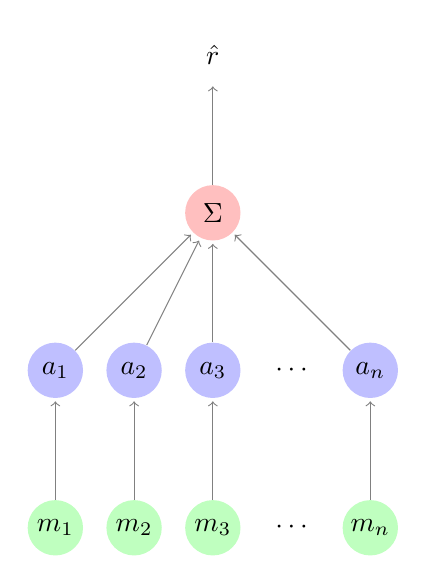
\begin{tikzpicture}[shorten >=1pt,->,draw=black!50, node distance=\layersep]
      \tikzstyle{every pin edge}=[<-,shorten <=2pt]
      \tikzstyle{node}=[circle,fill=black!25,minimum size=20pt,inner sep=0pt];
      \tikzstyle{method}=[node,fill=green!25];
      \tikzstyle{weight}=[node,fill=black!25];
      \tikzstyle{error}=[node,fill=blue!25];
      \tikzstyle{agg}=[node,fill=red!25];
      \tikzstyle{txt}=[node,fill=white];
       
      \node[method] (M1) at (0,-6) {$m_1$};      
      \node[method] (M2) at (1,-6) {$m_2$};         
      \node[method] (M3) at (2,-6) {$m_3$};         
      \node[txt]    (MS) at (3,-6) {$\cdots$}; 
      \node[method] (MN) at (4,-6) {$m_n$};
      \node[error]  (E1) at (0,-4) {$a_1$};      
      \node[error]  (E2) at (1,-4) {$a_2$};         
      \node[error]  (E3) at (2,-4) {$a_3$};         
      \node[txt]    (ES) at (3,-4) {$\cdots$}; 
      \node[error]  (EN) at (4,-4) {$a_n$};
      \node[agg]    (AG) at (2,-2) {$\Sigma$};
      \node[txt]    (RS) at (2,0)  {$\hat{r}$};
      
      \path (M1) edge (E1);
      \path (M2) edge (E2);
      \path (M3) edge (E3);
      \path (MN) edge (EN);
      \path (E1) edge (AG);
      \path (E2) edge (AG);
      \path (E3) edge (AG);
      \path (EN) edge (AG);
      \path (AG) edge (RS);
    \end{tikzpicture}
  \end{minipage} 
  \vspace{2em}
  \caption[Comparison of Aggregation and Adaption]{
    Comparison of aggregation and adaption:
    (left) modern aggregation approaches uses a set of pretrained weights
    to prioritize each modeling method.
    The weighted predictions are aggregated into a final prediction $\hat{r}$.
    (right) Stacked user modeling employs secondary modeling methods instead
    of weights. These estimate the accuracy of the initial method
    for the current user and item.
  }
  \label{fig:stack:comparison}
\end{figure}


